\chapter{Exigences non fonctionnelles}
Dans ce chapitre, les différentes exigences non fonctionnelles qui ont été sélectionnées seront explicitées. Pour rappel, de telles exigences décrivent les propriétés que le produit doit respecter. Pour ce faire, plusieurs de ces qualités ont été sélectionnées dans le modèle de Volere et seront présentées ci-dessous.

\section{Ergonomie et convivialité du produit}
SportEasy étant destiné à être une application sur smartphone, les couleurs, les interfaces et tout ce qui touche au visuel seront les premières choses que percevront les utilisateurs. Il est donc plus qu'important de définir quelque chose de plaisant et d'agréable afin de tout de suite accrocher le potentiel sportif et gagner le pas sur la concurrence. Afin de maximiser l'expérience de l'utilisateur et les chances de survie de l'application, il faut que les interfaces respectent certaines contraintes et que le packaging du produit soit attrayant.

\subsection*{Interface}
Cette application a pour vocation de configurer des séances sportives pour des utilisateurs aguerris ou non, comme il l'a déjà été mentionné plusieurs fois plus haut dans ce travail. Dès lors, il est nécessaire que son emploi soit rapide et intuitif et ne nécessite pas de lectures fastidieuses. Dès lors, il est important que la majorité de l'application soit graphique et compréhensible en un coup d'\oe il.\\

\'Etant donné que l'étude de partenariat n'a été menée que dans le cadre de la Belgique, notamment en Wallonie, il est normal que les interfaces soient définies, dans un premier temps, en français. Cependant, afin de toucher plus de monde, il est nécessaire de traduire ces interfaces le plus vite possible dans des langues plus accessibles (l'anglais, principalement, afin de devenir rapidement international).\\

La Figure \ref{fig:interfaces} montre des prototypes d'interfaces (qui ont d'ailleurs été plus détaillés dans le chapitre précédent). Ces IHM sont en accord avec la vision que le produit doit avoir : simples, sobres et efficaces.

\begin{figure}[!h]
	\centering
	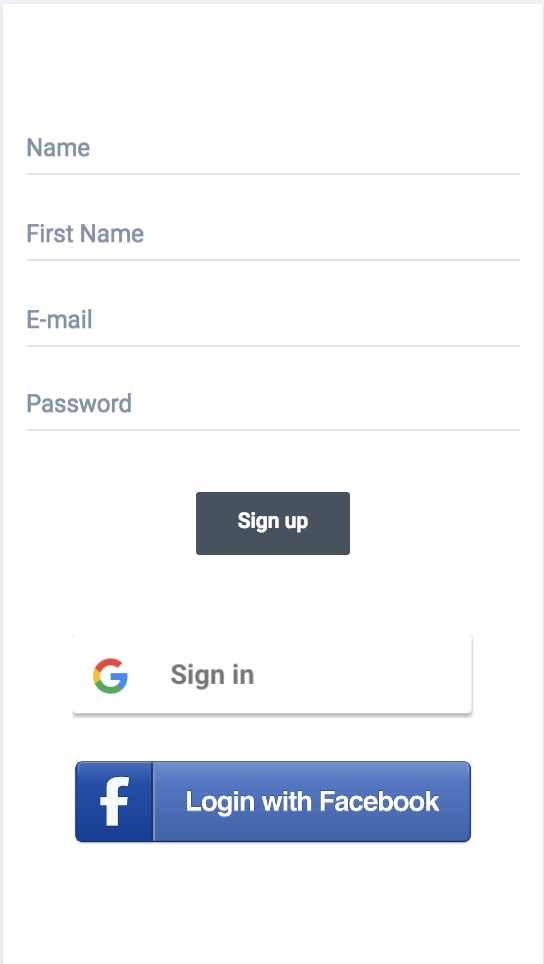
\includegraphics[scale=0.3]{ihms/inscription}
	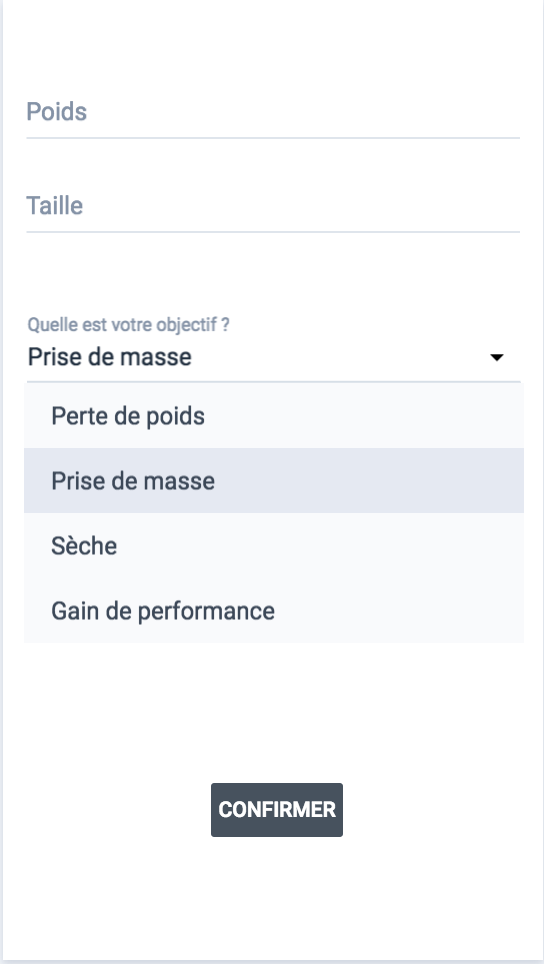
\includegraphics[scale=0.3]{ihms/caracteristiques}
	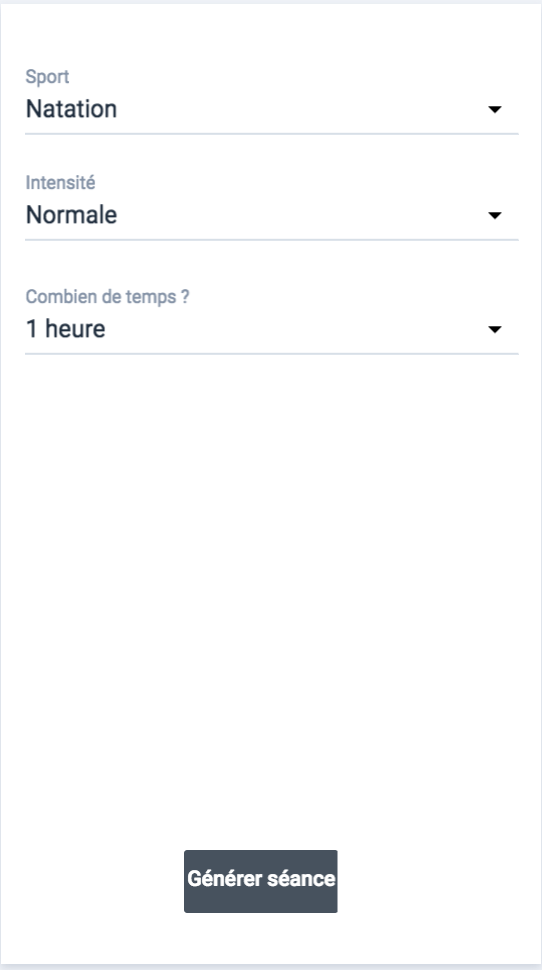
\includegraphics[scale=0.3]{ihms/seance}
	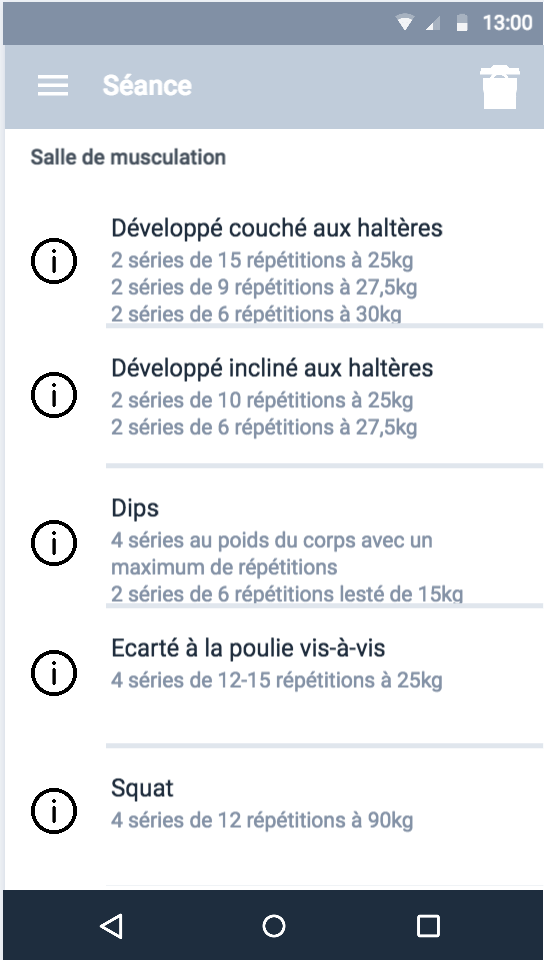
\includegraphics[scale=0.3]{ihms/normal_session}
	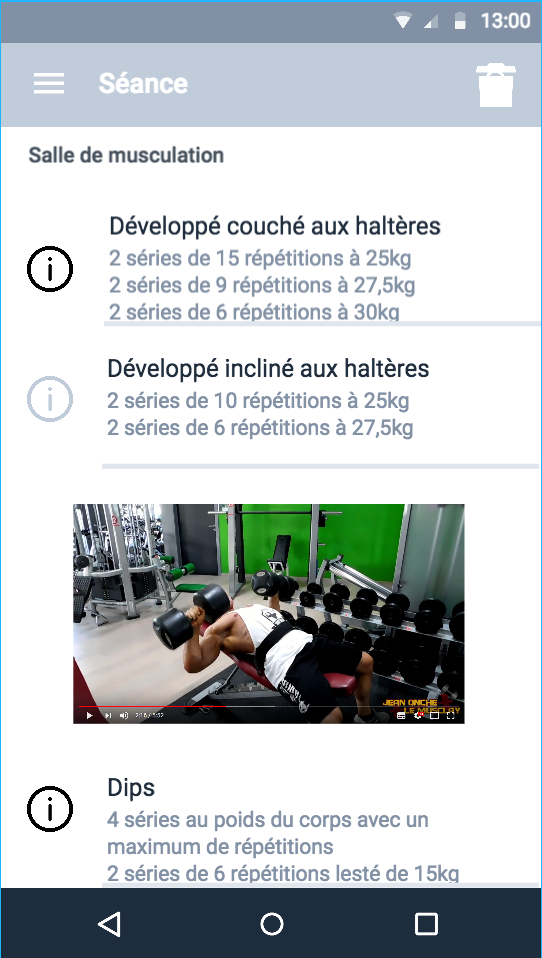
\includegraphics[scale=0.3]{ihms/get_information_about_exo}
	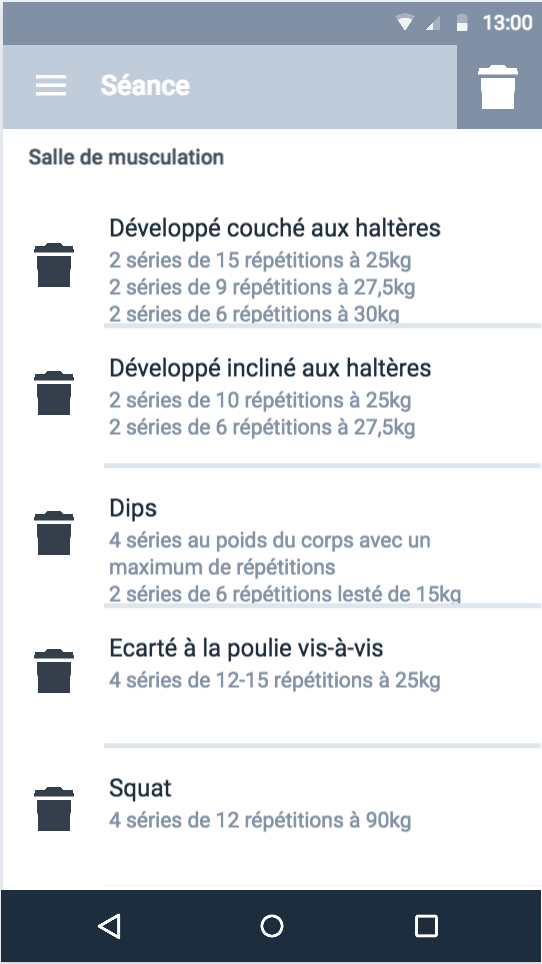
\includegraphics[scale=0.3]{ihms/remove_exo}
	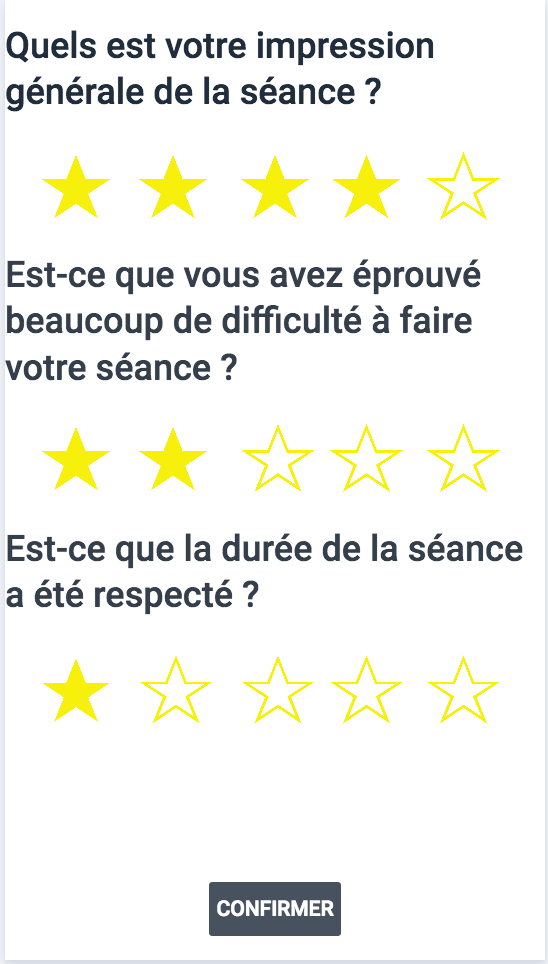
\includegraphics[scale=0.3]{ihms/rating_before_update}
	\caption{\label{fig:interfaces}Interfaces}
\end{figure}

\subsection*{Style et packaging du produit}
S'il est difficilement envisageable de définir un packaging pour une application mobile, il est néanmoins primordial que le produit respecte quelques conditions de style afin d'être un succès une fois lancé sur le marché.\\

Ainsi, le produit doit avoir l'air moderne et dynamique. Il est donc nécessaire que ce dernier respecte les dernières tendances en matière d'applications mobiles afin de se frayer un chemin aisé sur le marché et ne pas être désuet avant même d'avoir existé.\\

De même, bien que l'application soit destinée à toute personne souhaitant faire du sport, elle touchera rarement les enfants, qui nécessitent une attention particulière dans leur séance sportive de part leur croissance toujours bien active. Dès lors, l'application ne doit pas présenter de couleurs particulièrement \og flashy \fg{}.\\

Enfin, il est important que le produit suscite l'envie de faire du sport et stimule la motivation de l'utilisateur. Pour se faire, il doit employer un design frais, dynamique et énergétique tout en étant présenté de façon motivante. Le tout est que l'utilisateur ait envie de se lever pour faire du sport à peine ayant eu accès à l'application.

\section{Facilité d'utilisation et facteurs humains}
Le produit étant destiné à être utilisé par des personnes, non formées pour l'occasion, il est important de définir des exigences d'utilisation ; notamment la facilité d'emploi et d'apprentissage.

\subsection*{Facilité d'utilisation}
Les fonctionnalités du produit devraient être très simples. Comme mentionné précédemment, l'utilisateur souhaitant démarrer une séance de sport ne veut pas perdre 30 minutes de son temps à la configurer, ce qui lui laisserait effectivement moins de temps pour faire un entrainement. Dès lors, les points suivants doivent être respectés :\\

\begin{itemize}
	\item \textbf{Efficacité de la prise en main :} l'utilisateur doit être capable de prendre en main l'application et d'en utiliser toutes les fonctionnalités très rapidement. Dès lors, la prise en main sera plus longue (didacticiel d'emploi) et des pré-réglages seront stockés pour que la prise en main soit très rapide. Dès lors, après les 20 premières minutes d'utilisation de l'application, l'utilisateur est supposé savoir utiliser cette dernière parfaitement et rapidement.\\
	
	\item \textbf{Facilité de mémorisation :} l'application est supposée être intuitive pour être utilisée directement, sans besoin de formation particulière. Dès lors, il est considéré que l'utilisateur devrait être capable de se remémorer l'emploi d'une fonctionnalité après la 1\iere{} utilisation. Cependant, le produit étant destiné à des personnes de tout âge et de tout milieu, la limite sera fixée pour 3 utilisations de chaque fonctionnalité pour être certain que l'utilisateur se souvienne bien comment chaque fonctionnalité s'emploie.\\
	
	\item \textbf{Taux d'erreur :} l'utilisateur peut commettre des erreurs, cependant cela risque d'influencer en mal ses performances et donc biaiser l'application et sa fonctionnalité à proposer des séances adaptées. Ainsi, il existe 3 types d'erreurs, classées de bénignes à \og grave \fg{}. La première, c'est de se tromper dans la configuration de sa séance de sport. Il faut alors couper l'application et la relancer, cela fait perdre son temps à l'utilisateur. La seconde est le fait de se tromper dans le feedback fournit à la fin de la séance. Bien qu'il est rare de rencontrer ce cas, s'il se produit, l'adaptation de la séance ne sera pas efficace. Enfin, l'utilisateur peut couper l'application avant d'avoir terminé et validé sa séance. Dans ce cas, l'application ne pourra mettre à jour ses données et se comporter de façon efficace pour les prochains entrainements, ce qui est déplorable. Dès lors, il est nécessaire que le taux d'erreur global ne dépasse pas les 5\% en 1 mois d'utilisation afin de ne pas entacher le comportement normal du produit.\\
	
	\item \textbf{Satisfaction globale :} grâce aux feedbacks fournis par les fournisseurs d'applications mobiles (Play Store, Apple Store, ...), il est aisé de mesurer la satisfaction globale de l'utilisateur. Dès lors, il est important que l'application ne descende pas en dessous d'une satisfaction générale de 80\% endéans des 6 premiers mois.
\end{itemize}

\subsection*{Facilité d'apprentissage}
Comme expliqué ci-avant, le produit doit être facilement utilisable afin que l'utilisateur ne perde pas du temps précieux pour le configurer. De même, il faut tenir compte du fait que l'utilisateur normal est un adulte lambda qui ne doit présenter aucune qualification particulière pour employer l'application. Ainsi, un didacticiel sera mis en place afin que toute personne capable de lire puisse comprendre les étapes nécessaires à la configuration de la séance.\\

Très vite, le public doit être capable d'employer le produit sans devoir chercher. Au bout de 3 utilisations (répétition des mêmes mouvements), l'utilisateur doit être capable de configurer sa séance en toute maîtrise en 5 minutes maximum.

\subsection*{Facilité de compréhension et politesse}
Le produit n'est pas destiné à un professionnel du sport. Cela signifie qu'un amateur, un novice, peut souhaiter l'employer afin de s'entrainer. S'il connait certains termes techniques, tous les sens lui échappent sûrement. Cependant, il ne serait pas professionnel d'employer un vocabulaire infantile à la place. Pour s'assurer de la compréhension du vocabulaire sportif, des schémas ou vidéos explicatifs doivent être disponibles si l'utilisateur clique sur un des exercices.\\

Par ailleurs, il est aussi primordial de cacher les détails d'implémentation et de s'assurer qu'aucune exception n'apparaitra à l'utilisateur en tant que telle, dans un langage \og hérétique \fg{}. Toute exception devra être transformée en un message d'erreur clair et concis dans la langue de l'utilisateur.

\section{Fonctionnement du produit}
Ce chapitre traite des performances du produit quant à diverses données.

\subsection*{Rapidité et temps de latence}
Il est primordial que l'application soit rapide et que la latence ne soit pas perçue par l'utilisateur. Bien que le changement d'interfaces n'est pas paramétrable car il dépend des OS du smartphone, certaines fonctionnalités dépendent de la connexion internet. Dès lors, il ne faut pas que le chargement de ces fonctionnalités dépassent 2 secondes, sinon l'utilisateur risque de s'en désintéresser.

\subsection*{Fiabilité et disponibilité}
Le système doit être disponible toute l'année, 24h/24. Cependant, il est possible que les serveurs connaissent des pannes. L'application ne nécessite pas internet tout au long de son utilisation, mais certaines fonctionnalités en sont tributaires afin d'assurer leur bon déroulement. Dès lors, le produit peut être disponible 90\% du temps, et des mesures devront être mises en place afin de facilité la correction des problèmes et pannes dans des délais rapides.\\

Par ailleurs, étant donné la possibilité d'achats en ligne (pour des versions premium de l'application), il est nécessaire que le produit soit combiné à un service client. Ce service client doit être joignable durant les heures de bureau exception faite des congés légaux.

%- Robustesse et tolérance à un emploi erroné

\subsection*{Capacité de stockage et montée en charge}
Le système doit être capable de gérer un nombre important d'utilisateurs qui y accèdent en même temps. Cependant, ces accès aux serveurs sont partiels et ne nécessitent pas d'être connectés en permanence. Dès lors, il est rare que tous les utilisateurs requièrent un accès simultanés.\\

Il est raisonnable de penser que les jours d'affluence seront le week-end de 9h à 18h et qu'en semaine, les moments de pointe se feront plutôt de 12h à 14h ou en soirée (après 18h). Dans ces moments d'affluence, il a été considéré que le système devrait géré jusqu'à 200 accès simultanés. Le reste du temps, ceux-ci se feront pas aussi importants.\\

Le serveur s'occupera de traiter les données fournies par l'utilisateur (stockées sur son téléphone, pour des mesures de sécurité) et de renvoyer les réponses. Le serveur ne nécessite donc pas de conserver énormément de données et les réponses transférées sont très courtes. Les accès au système en ligne sont alors de durée très courte.

\section{Adéquation du produit avec son environnement}
Il sera décrit dans cette partie les exigences non fonctionnelles liées aux contraintes du projet.

\subsection*{Environnement technologique}
Bien que le produit n'ait aucune dépendance avec l'environnement physique spécifique, des contraintes technologiques ont été définies.\\

Comme mentionné précédemment, cette application sera déployée sur smartphone. Dès lors, elle devra être supportée principalement par les systèmes d'exploitation Android et iOS. Les Windows phones et Blackberry seront laissés de côté de par leur manque de popularité. La distribution et l'installation se feront alors au moyen des stores officiels qui redistribuent des applications.\\

L'application ne nécessite pas de matériel hardware supplémentaire que le téléphone, cependant, elle peut être couplée à des appareils connectés tels un cardio-fréquencemètre pour permettre la collecte de plus de données sur la séance de l'utilisateur.

\subsection*{Commercialisation}
Afin de commercialiser à grande échelle l'application, il a été défini dans le chapitre 2 qu'un partenariat serait mis en place avec de grandes salles de sport telles que Basic Fit. Dès lors, ces salles de sport devront mettre à disposition, à l'entrée de celles-ci, par exemple, des QR code permettant de se rendre sur le store et de télécharger et installer l'application.

\section{Maintenance et support du produit}
Cette partie traite de tout ce qui est maintenance, support et mise à jour du produit.

\subsection*{Exigences en matière de support}
Le produit va de paire avec un help desk. Celui-ci sera accessible par téléphone, email ou à l'aide d'une chat box en ligne. Cette aide sera prioritaire aux personnes ayant débloqués la version premium de l'application et permettra de répondre à diverses questions (utilisation, payements, problèmes techniques) ainsi que de faire remonter au niveau de la maintenance les problèmes soulevés n'ayant pas lieu d'être.

\section{Sécurité}
Cette partie traite de la confidentialité des données et de l'énergie dépensée pour lutter contre les attaques malveillantes.

\subsection*{Accès au système}
Seuls les administrateurs du système ont un droit d'accès et de regard concernant les données. Celui-ci doit s'effectuer de manière la plus sécurisée possible, afin d'éviter de laisser une porte ouverte aux personnes malveillantes.\\

Quant à l'accès physique des données, celui-ci ne peut se faire que pour les personnes en charge de la sécurité ainsi que les administrateurs du système. Celles-ci seront accédées à l'aide d'une double clé afin de ne pas permettre à une seule personne mal intentionnée d'y avoir accès.

\subsection*{Intégrité}
Comme le système ne stocke que très peu de données (essentiellement les comptes des utilisateurs et les données ayant servi au machine learning), c'est l'utilisateur qui fournit au système ce dont il a besoin pour lui répondre. Il doit alors vérifier que ce que lui donne l'utilisateur n'est pas compromis, dangereux ou abusif.\\

Afin d'éviter des problèmes de perte d'intégrité des données, le système doit posséder plusieurs backup de celles-ci. Les données ayant servi à l'entrainement du machine learning doivent se trouver sur un serveur hors ligne, présent dans un endroit qui ne présente que peu de risques de destruction physique. De même, les autres données doivent être sauvegardées périodiquement sur un serveur miroir. \'Etant donné la faible quantité de nouvelle donnée à stocker par jour, il est plus judicieux que cette sauvegarde se fasse toutes les semaines, après une période d'affluence.

\subsection*{Protection des données à caractère personnel}
Dans le but de protéger le plus les données à caractère personnel et d'être en adéquation avec le règlement à venir (RGPD ou équivalent étranger), la majorité des données nécessaire au bon fonctionnement de l'application seront stockées sur le téléphone de l'utilisateur. Ainsi, seules les données de compte (adresse mail, nom, prénom, mot de passe) seront conservées sur les serveurs. Ces données viseront à garantir un confort d'utilisation pour l'utilisateur, seront nécessaire en cas d'achat sur l'application et permettront d'affiner les partenariats avec les salles de sport, sans pour autant envahir l'utilisateur.\\

En ne stockant pas les données sur le serveur lié à l'application, un risque concernant les données très personnelles de milliers d'utilisateurs et transféré et devient alors la responsabilité de chaque personne de prendre soin de ses propres données.\\

De cette façon, l'application s'engage à ne pas stocker plus de données que nécessaires pour son bon fonctionnement et le confort d'expérience des utilisateurs.

\subsection*{Protection contre les infections}
Cette protection sera mise en place conformément aux mesures de sécurité décrites dans les ISO 27000 et suivants. Pour ce faire, l'organisation fera appel à des spécialistes de la sécurité qui mettront en place des mécanismes de protection logiciels et matériels.